
\documentclass{article}
\usepackage[utf8]{inputenc}
\usepackage{amsmath}
\usepackage{amssymb}
\usepackage{amsbsy}
\usepackage{graphicx}
\setcounter{secnumdepth}{-1}

%% notation

\newcommand{\D}{\ensuremath{\mathbf{D}}}
\newcommand{\sigmabf}{\ensuremath{\boldsymbol{\sigma}}}
\newcommand{\taubf}{\ensuremath{\boldsymbol{\tau}}}
\newcommand{\grad}{\ensuremath{\nabla}}
\renewcommand{\div}{\ensuremath{\nabla \cdot}}
\newcommand{\inner}[2]{\ensuremath{\left (#1, #2 \right)}}
\newcommand{\defeq}{\ensuremath{:=}}
\newcommand{\ddt}[1]{\ensuremath{\frac {\partial #1} {\partial t}}}
\newcommand{\dt}{\ensuremath{\Delta t}}



\newcommand{\stokes}{\ensuremath{\Omega_{f}}}
\newcommand{\stokesbdy}{\ensuremath{\Gamma_{f}}}
\newcommand{\darcy}{\ensuremath{\Omega_{p}}}
\newcommand{\darcybdy}{\ensuremath{\Gamma_{p}}}
\newcommand{\interface}{\ensuremath{\Gamma_{fp}}}
\newcommand{\nf}{\ensuremath{\mathbf{n}_f}}
\newcommand{\np}{\ensuremath{\mathbf{n}_p}}

% fluid test\trial functions
\newcommand{\uf}{\ensuremath{\mathbf{u}_f}}
\newcommand{\vf}{\ensuremath{\mathbf{v}_f}}
\newcommand{\up}{\ensuremath{\mathbf{u}_p}}
\newcommand{\vp}{\ensuremath{\mathbf{v}_p}}

% pressure test\trial functions
\newcommand{\pf}{\ensuremath{p_f}}
\newcommand{\pp}{\ensuremath{p_p}}
\newcommand{\wf}{\ensuremath{w_f}}
\renewcommand{\wp}{\ensuremath{w_p}}

% displacement test\trial functions
\newcommand{\disp}{\ensuremath{\boldsymbol{\eta}_p}}
\newcommand{\disptest}{\ensuremath{\boldsymbol{\xi}_p}}

% multiplier test\trial functions
\newcommand{\mult}{\ensuremath{\lambda_{\Gamma}}}
\newcommand{\multtest}{\ensuremath{\mu_{\Gamma}}}



\begin{document}

\title{Equations for system}
\maketitle


We follow \cite{ambartsumyan} very very closely.

\section{Domain}
Our domain $\Omega$ is $d=2 \text{ or } 3$-dimensional, and partitioned into \stokes and \darcy, with $\interface = \stokes \cap \darcy$ being the $(d-1)$-dimensional interface. The boundary $\partial \Omega$ is partitioned into $\stokesbdy = \partial \Omega \cap \partial \stokes$ and $\darcybdy = \partial \Omega \cap \partial \darcy$. We assume each region is connected, reasonably smooth and all that.

\section{Unknowns}
The unknowns of the system and the corresponding test functions are:

\begin{itemize}
\item \uf, \vf : free flow fluid velocity. Defined on \stokes.
\item \up, \vp : porous flow fluid velocity. Defined on \darcy.
\item \pf, \wf : free flow fluid pressure. Defined on \stokes.
\item \pp, \wp : porous flow fluid pressure. Defined on \darcy.
\item \disp, \disptest : displacement. Defined on \darcy.
\item \mult, \multtest : normal stress balance Lagrange multiplier. Defined on \interface. In \cite{ambartsumyan}, denoted $\lambda, \mu_h$.

\end{itemize}

\section{Parameters}

\begin{description}
\item[$\mu_f$] fluid viscosity (denoted $\mu$ in the \cite{ambartsumyan})
  
\item[$\lambda_p, \mu_p$] Lamé parameters. Denoted $\mu$ in \cite{ambartsumyan}.
\item[$\alpha$] Biot-Willis constant
\item[$K$] Permeability tensor. Symmetric, bounded, positive definite. I take it to be scalar.
\item[$\alpha_{BJS}$] Friction coefficient
\end{description}

\section{Notation}
\begin{itemize}
\item \nf, \np are the outward unit normal vectors to $\partial \stokes, \partial \darcy$. 
\item $\taubf_{f, j}, j = 1, \ldots, d-1$ is an orthogonal system of unit tangent vectors at \interface.
\item $\D(\mathbf{v}) \defeq \frac 12 (\grad \mathbf{v} + \grad \mathbf{v}^T)$
\item $\sigmabf_f(\uf, \pf) \defeq -\pf \mathbf{I} + 2 \mu_f \D(\uf)$
\item $\sigmabf_p(\disp, \pp) \defeq \lambda_p (\div \disp) + 2 \mu_p \D(\disp) - \alpha \pp \mathbf{I} $
  
\item $a_f(\uf, \vf) = \inner{2\mu \D(\uf)} {\D(\vf)}_{\stokes}$
\item $a_p^d(\up, \vp) = \inner{\mu K^{-1}\up} {\vp}_{\darcy}$
\item $a_p^e(\disp, \disptest) = \inner{\mu_p \D(\disp)} {\D(\disptest)}_{\darcy} + \inner{\lambda_p \div \disp} {\div \disptest}_{\darcy}$
  
\end{itemize}


\section{Strong formulation}
These are all ignoring body force and source terms. So it's okay to put stuff on the right hand sides if you want to.

Stokes (applies in \stokes):
\begin{subequations}
  \begin{align}
    - \div \sigmabf_f (\uf, \pf) = 0    \label{eq:stokes_stress} \\
    \div \uf = 0    \label{eq:stokes_conservation}
  \end{align}
\end{subequations}

Darcy (applies in \darcy):
\begin{equation}
    \up = - \frac {K} {\mu} \grad \pp     \label{eq:darcy}
  \end{equation}

  
Biot (applies in \darcy):
\begin{subequations}
  \begin{align}
    - \div \sigmabf_p (\disp, \pp) = 0     \label{eq:biot_stress} \\
    \ddt{} \left ( s_0 \pp + \alpha \div \disp \right ) + \div \up = 0    \label{eq:biot_conservation}
  \end{align}
\end{subequations}
\section{Interface conditions}

Conservation of mass:
\begin{equation}
\uf  \cdot \nf + \left ( \ddt{\disp} + \up \right ) \cdot \np = 0  \label{eq:massconservation}
\end{equation}
Balance of stress (will be enforced using \mult):
\begin{equation}
  -(\sigmabf_f \nf) \cdot \nf = \pp, \hspace{0.02\linewidth} \sigmabf_f \nf + \sigmabf_p \np \ = 0, \:  \label{eq:stressbalance}
\end{equation}
BJS condition:
\begin{equation}
  -(\sigmabf_f \nf) \cdot \taubf_j = \frac {\mu_f \alpha_{BJS}} {\sqrt{K}} \left ( \uf - \ddt{\disp} \right ) \cdot \taubf_j
  \label{eq:BJS}
\end{equation}
Pressure difference across vessel wall:
\begin{equation}
  \pf - \pp = C
  \label{eq:pressurejump}
\end{equation}
\cite{ambartsumyan} does not use condition \ref{eq:pressurejump}.



\section{Boundary conditions}
In their numerical experiment (section 7.2), \cite{ambartsumyan} use the domain shown in figure \ref{fig:ambartsumyandomain}
\begin{figure}[h]
  \centering
  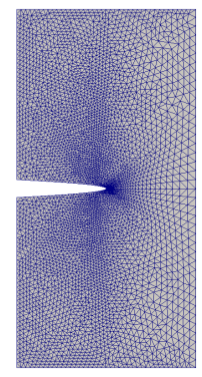
\includegraphics[width=0.15\textwidth]{img/ambartsumyandomain.png}
  \label{fig:ambartsumyandomain}
  \caption{Darcy domain from \cite{ambartsumyan}. Stokes domain is the removed 'finger'.}
\end{figure}
The Darcy boundary \darcybdy is partitioned into the left part $\darcybdy^{\text{L}}$ and the remainder $\darcybdy^{\neg \text{L}}$ in the obvious way. Physically, I think $\darcybdy^{\text{L}}$ is above ground and the other part is below ground or something.

As boundary conditions, they use:
\begin{itemize}
\item $\uf = 10 \nf$ on \stokesbdy
\item $\up \cdot \np = 0$ on $\darcybdy^{\text{left}}$
\item $\pp = 1000$ on $\darcybdy^{\neg \text{left}}$
\item $\disp \cdot \np = 0$ on $\darcybdy^{\neg \text{left}}$
\item $(\sigmabf_p \np) \cdot \taubf_p = 0$ on $\darcybdy^{\neg \text{left}}$
  
\end{itemize}
\section{Variational formulation}
Having used a backward Euler discretization of the time derivative, \cite{ambartsumyan} obtain the following variational formulation

\begin{subequations}
  \begin{align}
    a_f (\uf, \vf) &+ a_p^d(\up, \vp) + a_p^e(\disp, \disptest)  + a_{BJS}\left (\uf, \frac {\disp} {\dt}; \vf, \disptest \right) \label{eq:varform1} \\
    & + b_f(\vf, \pf) + b_p(\vp, \pp) + \alpha b_p(\disptest, \pp)   \nonumber \\
    & + b_{\Gamma}(\vf, \vp, \disptest; \mult) \nonumber \\ &= a_{BJS}\left (\uf, \frac {\disp^{n-1}} {\dt}; \vf, \disptest \right)  \nonumber \\ 
    \inner{s_0 \frac {\pp} {\dt}}{\wp}_{\darcy}  &- \alpha b_p\left ( \frac{\disp} {\dt}, \wp \right ) - b_p(\up, \wp) - b_f(\uf, \wf) \label{eq:varform2}
    \\ &= \inner{s_0 \frac {\pp^{n-1}} {\dt}}{\wp}_{\darcy} - \alpha b_p\left ( \frac {\disp^{n-1}} {\dt}, \wp \right )_{\darcy}\nonumber \\
    b_{\Gamma}\left (\uf, \up; \disp \dt \right ) &= b_{\Gamma}\left (\uf, \up; \disp^{n-1} \right ) \label{eq:varform3}
  \end{align}
\end{subequations}

Here the unknowns with no superscript mean the unknowns at time $n$ (e.g. $\uf = \uf^n$).





\section{Thoughts}
\begin{itemize}
\item Kent offered very gentle scepticism about using a 3-field formulation, and suggested not having \up as an unknown, using $\up = \grad \pp$ to remove it. I thought \cite{ambartsumyan} had some opinion on this, but on closer reading I can't find it, so maybe that's from another article. I should read up on this.
\item If I want to use \ref{eq:pressurejump}, I need to drop an interface condition. The most reasonable thing to drop seem to be the first part of \ref{eq:stressbalance}, because they both effectively specify \pp. But I don't like the BJS condition because it has too many letters, so I'd like an excuse to drop that instead.
  
 
\end{itemize}


\bibliographystyle{amsalpha}
\begin{thebibliography}{99}
\bibitem{ambartsumyan}
{\sc Ambartsumyan, Ilona, et al. }, {\em "A Lagrange multiplier method for a Stokes-Biot fluid-poroelastic structure interaction model." }, arXiv preprint arXiv:1710.06750 (2017).
  
\end{thebibliography}

\end{document}
